\documentclass[xcolor=dvipsnames]{beamer} 
\setbeamertemplate{blocks}[rounded][shadow=false]

\usetheme{Madrid}

\setbeamertemplate{items}[square]

\usepackage{float}
\usepackage[brazil]{babel}
\usepackage[utf8]{inputenc}

\usepackage{graphicx}
\usepackage{url}
\usepackage{float}     % para forçar a localizaçao das figuras (usando H no posicionamento, =Here)

\usepackage{scalefnt}
\usepackage{ragged2e}
\usepackage{etoolbox}
\usepackage{enumerate}
\usepackage{verbatim}

\usepackage{subcaption} 

\usepackage{tikzsymbols} %emoticons
\usepackage{xparse}% http://ctan.org/pkg/xparse
\NewDocumentCommand{\ceil}{s O{} m}{%
  \IfBooleanTF{#1} % starred
    {\left\lceil#3\right\rceil} % \ceil*[..]{..}
    {#2\lceil#3#2\rceil} % \ceil[..]{..}
}

\newcommand{\aspas}[1]{``#1''}

\let\olditem=\item% 
\renewcommand{\item}{\olditem \justifying}%

\hyphenation{LogNormal}

%\usetheme{Antibes}
%\usetheme{Berlin}

\title[Introdução à Simulação - CComp]{Introdução à Simulação}
\subtitle{Trabalho Prático 03 - Implementação e Análise de um Modelo de Simulação de uma Fundição}
\author[César, Ramos, Guimarães]
{João Paulo Fernandes Cerqueira César, Natanael Ramos, \\Rodolfo Labiapari Mansur Guimarães}
\institute[IFMG]{Instituto Federal de Educação, Ciência e Tecnologia de Minas Gerais (IFMG) \\ - \textit{campus} Formiga}
\date[\today]{\today}

\begin{document}
\frame{\titlepage}

%\AtBeginSection[] 
%{
%	\begin{frame}[allowframebreaks]
%	\frametitle{Sumário}
%	\tableofcontents[currentsection]
%	\end{frame}
%}

\section{Introdução}
\begin{frame}{}
	\centering
	\Huge \color{blue} \textbf{Introdução}
\end{frame}


\begin{frame}{Introdução}
	\begin{itemize}
		\item Foi \textbf{construído} um modelo de simulação de uma fundição situada na cidade Itaguara;
		      \bigskip
		      			
		\item Limitou-se o escopo de modelagem à produção da peça piloto do lote;
		      			
		      \bigskip
		      			
		\item Etapas:
		      \begin{enumerate}
		      	\item Visita à fundição para entrevista com um sócio do empreendimento, coletando;
		      	      \begin{itemize}
		      	      	\item Atividades envolvidas no processo;
		      	      	\item Estimação de durações das atividades;
		      	      	\item Possíveis filas;
		      	      	\item Ligação entre as atividades do processo.
		      	      \end{itemize}
		      	      				
		      	      \bigskip
		      	      				
		      	\item Construção do Diagrama Cíclico de Atividades;
		      	      				
		      	      \bigskip
		      	      				
		      	\item Implementação do Modelo.
		      \end{enumerate}
		      			
	\end{itemize}
\end{frame}

\section{Descrição Textual}
\begin{frame}{}
	\centering
	\Huge \color{blue} \textbf{Descrição Textual}
\end{frame}
\subsection{Texto Descritivo Detalhado}
	
\subsubsection{Departamento de Compra (a)}
\begin{frame}{Departamento de Compra (a)}
	\begin{itemize}
		\item Numa fundição produz-se vários tipos de peças de acordo com os requisitos do cliente.
		      				
		      \bigskip
		      				
		\item Nela, chega clientes no Departamento de Compra para realizar o pedido. A chegada de pedidos segue uma distribuição \texttt{normal de média 120 e desvio padrão 40 minutos}.
		      				
		      \bigskip
		      				
		\item O pedido é processado e enviado a linha de produção no setor de expedição. O tempo de processar e enviar para o setor de expedição segue uma \texttt{distribuição triangular de mínimo 30, moda 40 e máximo 180 minutos} e é feito pela única secretária existente no local.
	\end{itemize}
\end{frame}
	
\subsubsection{Setor de Expedição (b)}
\begin{frame}{Setor de Expedição (b)}
	\begin{itemize}
		\item {\color{red} Existe apenas 1 funcionário para a análise de expedição.}
		      				
		      \bigskip
		      				
		\item Existe a análise de composições químicas para a fabricação e verificação do que existe em estoque no qual segue uma \texttt{distribuição triangular de mínimo 15, moda 30 e máxima de 180 minutos}.
		      				
		      \bigskip
		      				
		\item Verificar a data de entrega do material, o que é, qual matéria-prima principal ele é feito, normal e outros ações básicas segue uma \\\texttt{distribuição uniforme de no mínimo 15 e no máximo 45\\ minutos}.
		      				
		      \bigskip
		      				
		\item Após isso, realiza-se o estudo, elaboração e planejamento da sua produção no qual segue uma \texttt{distribuição normal de média 30 e desvio padrão 12 minutos}.
		      				
		      \bigskip
		      				
		\item Após isso, este é repassado para a linha de produção no setor de modelagem.
	\end{itemize}
\end{frame}
		
\subsubsection{Setor de Modelagem (c)}
\begin{frame}{Setor de Modelagem (c)}
	\begin{itemize}
		\item{\color{red}Existe 1 funcionário para a realização de todos os procedimentos da modelagem.}
						
		\bigskip
						
		\item Na modelagem da produção, deve-se verificar se no depósito de modelagem existe um modelo arquivado para a execução deste produto, sabe-se que este tem uma \texttt{distribuição uniforme de mínimo 15 e máximo 25 minutos}.
		      				
		      \bigskip
		      				
		\item {\color{red} Sabe-se também que 70\% dos produtos a serem enviados para a linha de produção já existem moldes na empresa para serem reutilizados. Caso já tenha, utiliza este. Caso contrário, precisa criar um modelo no qual segue uma \texttt{distribuição triangular de mínimo 8 horas, moda 3 dias e máximo de 5 dias} para a conclusão.}
	\end{itemize}
\end{frame}
		
\begin{frame}{Setor de Modelagem (c)}
	\begin{itemize}
		\item Com o modelo em mãos, realiza o rastreamento (Rastreabilidade,\\ histórico) do produto, ou seja, o que já foi feito pela empresa de algo semelhante, o material, etc. Isso segue uma \texttt{distribuição triangular de mínimo 2, moda 30 e máximo de 180 minutos}.
		      				
		      \bigskip
		      				
		\item Após recolhido todas as informações necessárias, essas são colocadas junto com cada peça para sua identificação ao longo do processo de produção, isto segue uma \texttt{distribuição triangular de mínimo 5, moda 10, e máximo 40 minutos}.
		      				
		      \bigskip
		      				
		\item Após isso está é levada para a linha de produção.
	\end{itemize}
\end{frame}
		
\subsubsection{Setor de Produção (d)}
\begin{frame}{Setor de Produção (d)}
	\begin{itemize}
		\item A peça é levada para ser preenchida de areia no qual segue uma \\\texttt{distribuição normal com média 4 e desvio padrão de 2 \\minutos}.
		      				
		      \bigskip
		      				
		\item Em seguida leva-se \texttt{10 minutos} para realizar a identificação do material a ser fundido, temperatura máxima, horário de tirá-la do forno, entre outros.
		      				
		      \bigskip
		      				
		\item {\color{red} Um funcionário é encarregado dos dois procedimentos ditos acima.
			      					
			      \bigskip
			      					
			\item 30\% são feitas a máquina, 40\% a mão e 30\% feitas a resina sendo que na resina 10\% são feitas com caixote e 20\% são feitas sem o caixote totalizando 100\% das peças produzidas pela empresa.}
	\end{itemize}
\end{frame}
		
		
\subsubsection{Setor de Produção (d)}
\begin{frame}{Setor de Produção (d)}
	\begin{itemize}
		\item O processo da máquina faz 1 peça por minuto e realiza o trabalho de peças pequenas;
		      				
		      \bigskip
		      				
		\item O processo manual faz 1 peça a cada 8 minutos {\color{red}(onde trabalha o segundo funcionário. Este é encarregado somente esta função)};
		      				
		      \bigskip
		      				
		\item Por resina utiliza-se somente peças de grande porte. Na resina existe as produções:
		      				
		      \begin{itemize}
		      	\item Sem caixote que segue uma \texttt{distribuição triangular de mínimo 20, moda 24 e máximo de 28 minutos};
		      	      					
		      	      \bigskip
		      	      					
		      	\item Com caixote que utiliza exatamente 24 minutos para operar e mais 7 minutos para limpeza quando acabar o processo.
		      \end{itemize}
	\end{itemize}
\end{frame}
		
\subsubsection{Finalização da peça (e)}
\begin{frame}{Finalização da peça (e)}
	\begin{itemize}
		\item{\color{red} Existem 2 funcionário para este setor.}
						
		\bigskip
						
		\item Após construir o produto, ele passa por uma finalização. Nela é realizado o Checkout/Limpeza e Acabamento.
		      				
		      \bigskip
		      				
		\item O Checkout e limpeza no qual é feito uma desmolda da peça e retira a areia que sobra no qual volta para o sistema. Isso dura cerca de uma \texttt{distribuição uniforme de mínimo 2 e máximo 3 minutos}. Para produtos feitos com o método de resina, {\color{red} existe 1 funcionário por conta de realizar este serviço no qual} necessita de \texttt{18 horas} para sua conclusão. {\color{red} O outro, cuida de todo o resto do setor inclusive o trabalho manual.}
	\end{itemize}
\end{frame}
		
		
\subsubsection{Finalização da peça (e)}
\begin{frame}{Finalização da peça (e)}
	\begin{itemize}
		\item Já no acabamento é feito o resfriamento da peça que segue uma \texttt{distribuição normal de 1 hora com desvio padrão de 30\\ minutos para o manuseio posterior}.
		      				
		      \bigskip
		      				
		\item Após resfriada/desaquecido, a peça é esmerilada no tempo de \texttt{10 minutos} e depois segue para a rebarbação. Na rebarbação, é possível ser feita manualmente ou por máquina. Sabe-se que:
		      \begin{itemize}
		      	\item 60\% das peças são feitas manualmente sendo esta uma \texttt{distribuição triangular de mínimo 3, moda 5 e máxima 10 minutos}; 
		      	      					
		      	      \bigskip
		      	      					
		      	      					
		      	\item 40\% feitas à máquina seguindo uma \texttt{distribuição uniforme \\de mínimo 1 e máximo 3 minutos}.
		      \end{itemize}
	\end{itemize}
\end{frame}
		
\subsubsection{Setor de Qualidade (f)}
\begin{frame}{Setor de Qualidade (f)}
	\begin{itemize}
		\item Depois é feito uma análise visual na própria empresa no qual leva 2 minutos.
		      				
		      \bigskip
		      				
		\item Envia-se uma peça chamada corpo de prova para uma empresa terceirizada ou mesmo o SENAI para que eles realizem testes como Composição Química, Alongamento, Dureza entre outros. Isto segue uma \texttt{distribuição triangular de mínimo 3, moda 4 e máximo 7 \\dias}.
		      				
		      \bigskip
		      				
		\item Após \textbf{todos} os testes realizados, o produto é liberado de volta para a produção e geração de documentos. {\color{red}No modelo, colocou-se 1 funcionário para estas atividades para representar que ambas devem ser executadas para que os processos possam continuar}
	\end{itemize}
\end{frame}
		
\subsubsection{Continuação Produção (g)}
\begin{frame}{Continuação Produção (g)}
	\begin{itemize}
		\item O produto pode, se for um requisito no ato da compra do serviço, ser pintado. O processo de pintura ocorre em 90\% dos produtos fabricados e leva uma \texttt{distribuição normal de 1 minutos com desvio padrão de 2 minutos}.
		      				
		      \bigskip
		      				
		\item {\color{red} Apenas 1 funcionário fica a par de trabalhar na pintura.}
		      				
		      \bigskip
		      				
		\item Após isso, o produto é levado para o depósito.
	\end{itemize}
\end{frame}
		
\subsubsection{Geração dos documentos do produto (h)}
\begin{frame}{Geração dos documentos do produto (h)}
	\begin{itemize}
		\item A geração de documentos é um cargo responsável pelo desenvolvimento de certificados, normas e documentação de propriedades como composição química, dureza, alongamento, tração e entre outros. A distribuição desta operação segue uma \texttt{distribuição uniforme com mínimo 1 dia e máximo 3 dias}.
		      				
		      \bigskip
		      				
		\item {\color{red} Uma assistente fica a par para realizar tais tarefas}.
	\end{itemize}
\end{frame}
		
\section{Modelo ACD}

\begin{frame}{}
	\centering
	\Huge \color{blue} \textbf{Modelo de Diagrama Cíclico de Atividades}
\end{frame}
		
\begin{frame}{DCA - Departamento de Compra}
	\begin{figure}[H]
		\centering
		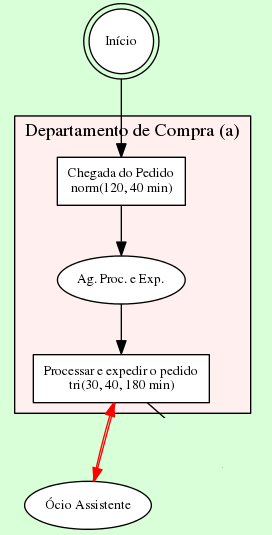
\includegraphics[height=0.865\textheight]{img/a.png}
	\end{figure}
\end{frame}
	
\begin{frame}{DCA - Setor de Expedição}
	\begin{figure}[H]
		\centering
		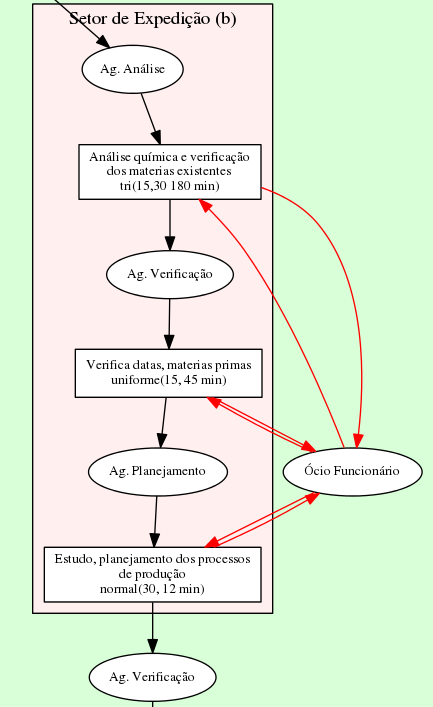
\includegraphics[height=0.865\textheight]{img/b.png}
	\end{figure}
\end{frame}
	
\begin{frame}{DCA - Setor de Modelagem}
	\begin{figure}[H]
		\centering
		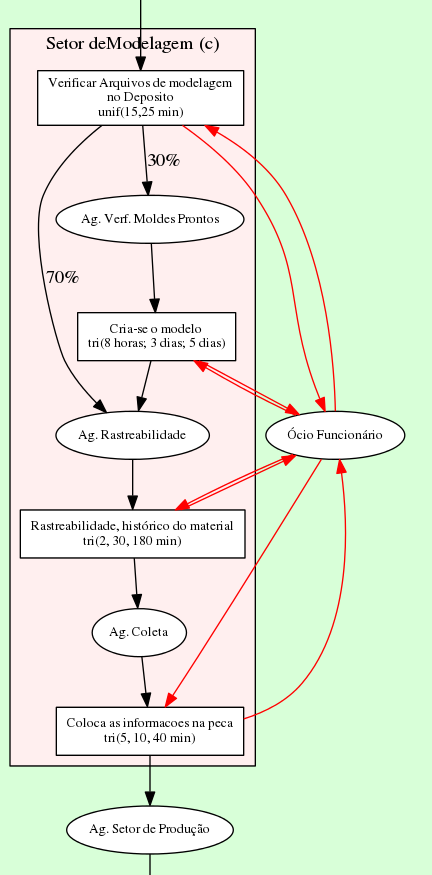
\includegraphics[height=0.865\textheight]{img/c.png}
	\end{figure}
\end{frame}
	
\begin{frame}{DCA - Setor de Produção}
	\begin{figure}[H]
		\centering
		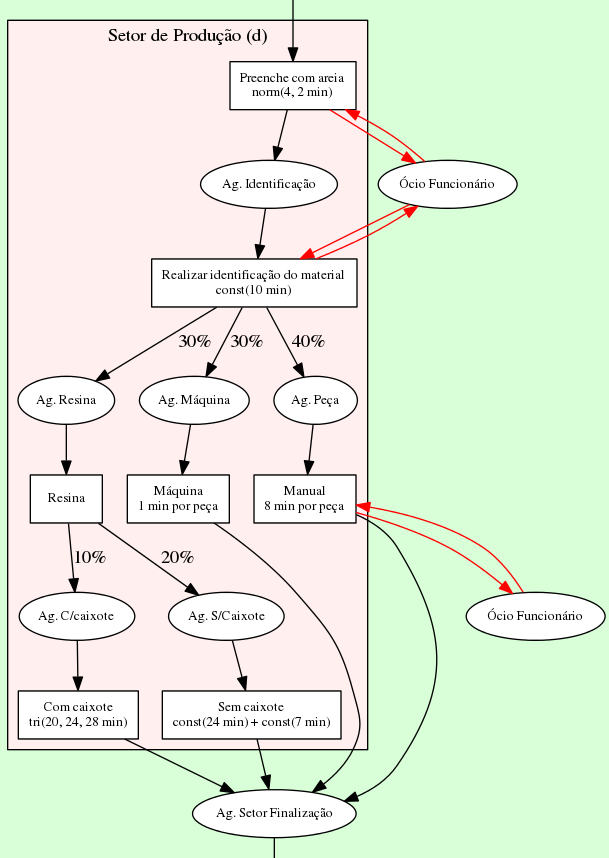
\includegraphics[height=0.865\textheight]{img/d.png}
	\end{figure}
\end{frame}
	
\begin{frame}{DCA - Finalização do Produto}
	\begin{figure}[H]
		\centering
		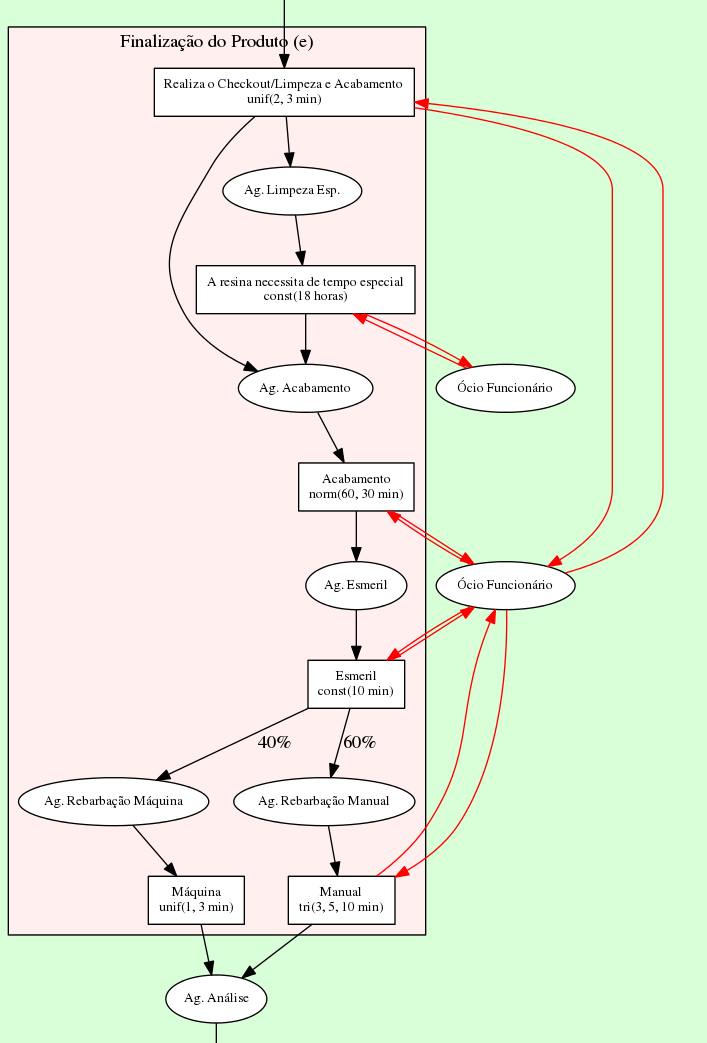
\includegraphics[height=0.865\textheight]{img/e.png}
	\end{figure}
\end{frame}
	
\begin{frame}{DCA - Setor de Qualidade}
	\begin{figure}[H]
		\centering
		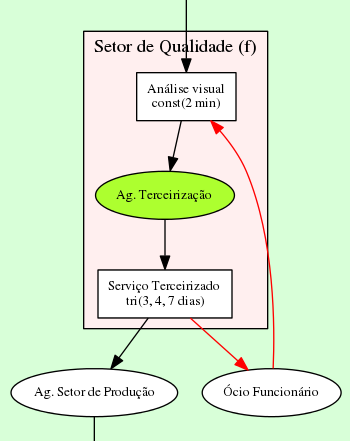
\includegraphics[height=0.865\textheight]{img/f.png}
	\end{figure}
\end{frame}
	
\begin{frame}{DCA - Setor de Continuação do Produto}
	\begin{figure}[H]
		\centering
		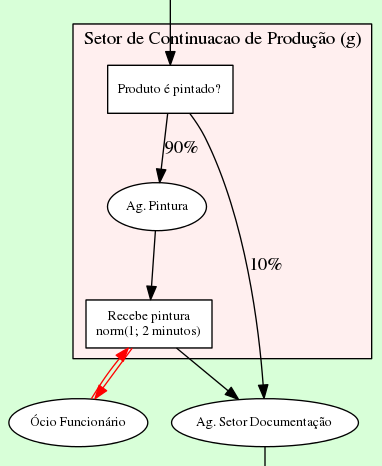
\includegraphics[height=0.865\textheight]{img/g.png}
	\end{figure}
\end{frame}
	
\begin{frame}{DCA - Setor de Geração de Documento}
	\begin{figure}[H]
		\centering
		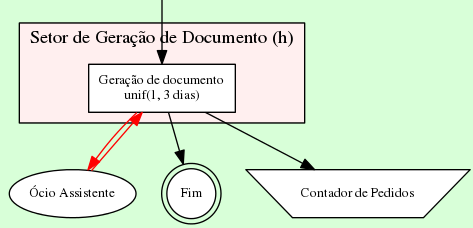
\includegraphics[width=1.0\textwidth]{img/h.png}
	\end{figure}
\end{frame}	

\section{Definições da Simulação}

\begin{frame}{}
	\centering
	\Huge \color{blue} \textbf{Definições da Simulação}
\end{frame}
	
\subsection{Indicador de Desempenho}
	
\begin{frame}{Indicador de Desempenho}
	\begin{itemize}
		\item Tempo médio de espera na fila do Serviço de Terceiros;
		      			
		      \bigskip
		      			
		\item É a atividade mais demorada: {\tt distribuição triangular de mínimo 3, moda 4 e máximo 7 dias};
		      			
		      \bigskip
		      			
		      \begin{block}{Contratar mais serviços de empresas terceirizadas, reduz o tempo de espera na fila de Serviços Terceirizados?}
		      	Talvez o ato de pagar um pouco mais caro por mais serviços possa gerar mais lucro pelo fato de diminuir o gargalo na fila de espera do serviço de terceiros, levando ao atendimento de mais pedidos.
		      \end{block}
		      			
	\end{itemize}
\end{frame}
	
\subsection{Cenários}
	
\begin{frame}{Cenários}
\fontsize{10pt}{7.2}\selectfont
	\begin{itemize}
		\item Intervalo de confiança de 95\% com $\alpha$ de 0.05;
        \medskip
		\item Precisão desejada $h*$ de 120 minutos;
        \medskip
		\item \textbf{Replicações}: inicialmente foram executadas $n=1.000.000$ replicações, na comparação entre cenários, verificou-se que eram necessárias mais $n*=466.188$ replicações para alcançar a precisão desejada, totalizando $n=1.466.188$;
        \medskip
		\item \textbf{Tempo}: 6 meses, considerando 8 horas trabalhadas por dia, 5 dias por semana e 20 dias por mês;
        \medskip
		\item \textbf{Quantidade de Pedidos}: 15;
        \medskip
		\item \textbf{Duração das atividades:} Manteve-se as especificadas no ACD original;
        \medskip
		\item \textbf{Variabilidade}: Para variação dos cenários, foi alterada a disponibilidade dos funcionários;
        \medskip
		\item \textbf{Cenário \textit{default} (CD)}: Manteve-se as configurações do ACD.
	\end{itemize}
\end{frame}
	
\section{Metodologia}

\subsection{Ambiente}
	
\begin{frame}{}
	\centering
	\Huge \color{blue} \textbf{Ambiente}
\end{frame}
	
\begin{frame}{Ambiente de Desenvolvimento}
	\begin{itemize}
		\item Linguagem de Programação Java, com o paradigma de Orientação a Objetos;
        \bigskip
		\item Versão do Java: 1.8.0\_45;
        \bigskip
		\item Sistema Operacional Linux, \textit{kernel} de versão: {\tt 3.16.0-38-generic};
        \bigskip
		\item Distribuição Linux Mint, versão 17.2;
        \bigskip
		\item IDE (\textit{Integrated Development Environment}) Intellij IDEA com licença para estudante.
	\end{itemize}
\end{frame}
	
\begin{frame}{Ambiente de Experimentação}
	\begin{itemize}
		\item Sistema Operacional Linux, \textit{kernel} de versão: {\tt 3.16.0-38-generic};
        \bigskip
		\item Distribuição Linux Mint, versão 17.2;
        \bigskip
		\item Processador Intel Core i7-4500U com \textit{clock} de 1.80GHz;
        \bigskip
		\item Memória RAM DDR3 de 7.7GB.
	\end{itemize}
\end{frame}
	
\subsection{Implementação Computacional}
		
\begin{frame}{}
	\centering
	\Huge \color{blue} \textbf{Implementação Computacional}
\end{frame}
	
\begin{frame}{Implementação Computacional}
\fontsize{10pt}{7.2}\selectfont
	\begin{itemize}
		\item Possui como principais elementos:
        \medskip
		      \begin{itemize}
		      	\item \textit{\textbf{clock}};
                \medskip
		      	\item \textbf{FEL} (Fila de Eventos Futuros, do inglês \textit{Future Event List});
                \medskip
		      	\item Filas de atividades;
                \medskip
		      	\item Entidades;
                \medskip
		      	\item Eventos.
		      \end{itemize}
		      \bigskip
		\item Possui como principais fases:
        \medskip
		      \begin{itemize}
		      	\item Inicialização;
		      	      \medskip
		      	\item Nascedouro;
		      	      \medskip
		      	\item Período de simulação;
		      	      \begin{itemize}
		      	      	\item Geração de eventos;
		      	      	      \medskip
		      	      	\item Execução de atividades.
		      	      \end{itemize}
		      	      \medskip
		      	\item Coleta final de estatísticas.
		      \end{itemize}
	\end{itemize}
\end{frame}
	
\begin{frame}{Implementação Computacional - Bibliotecas}
	\begin{itemize}
		\item Foi utilizada a biblioteca \textit{math commons} do Apache sob a licença Apache License 2.0;
		      			
		      \bigskip
		      			
		\item Geração de variáveis aleatórias segundo distribuições de probabilidade:
		      \begin{itemize}
		      	\item Triangular;
		      	      \bigskip
		      	\item Uniforme Inteira;
		      	      \bigskip
		      	\item Normal.
		      \end{itemize}
		      			
		      \bigskip
		      			
		\item Para geração de números aleatórios, utilizou-se o algoritmo Mersenne Twister \footnote{\url{http://www.math.sci.hiroshima-u.ac.jp/~m-mat/MT/emt.html}}.
	\end{itemize}
\end{frame}
	
\begin{frame}{Implementação Computacional - Clock}
	\begin{itemize}
		\item Marco de tempo da simulação;
		\bigskip
		\item É \textbf{sempre} incrementado em $n$ unidades, onde $n$ é o tempo de término do último evento reconhecido;
        \bigskip
		\item Serve como critério de parada para a simulação.
	\end{itemize}
\end{frame}
	
\begin{frame}{Implementação Computacional - Entidades}
	\begin{itemize}
		\item Pedido possui:
        \bigskip
		      \begin{itemize}
		      	\item Identificador;
		      	      \bigskip
		      	\item Marcador de tempo em que entrou na fila, para calcular o tempo médio de espera de cada fila.
		      \end{itemize}
		      \bigskip
		\item Demais entidades (funcionário e serviços terceirizados) são apenas contadores.
	\end{itemize}
\end{frame}
	
\begin{frame}{Implementação Computacional - Eventos}
\fontsize{10pt}{7.2}\selectfont
	\begin{itemize}
		\item Cada evento possui:
        \medskip
		      \begin{itemize}
		      	\item O tipo de evento;
		      	      \bigskip
		      	\item O evento gerador;
		      	      \bigskip
		      	\item Identificador do respectivo pedido;
		      	      \bigskip
		      	\item O tempo de término do evento.
		      	      \bigskip
		      \end{itemize}
		\item O tempo de término de cada evento é calculado por: $$ clock + dist.sample(parametros) $$
		\item Onde:
        \medskip
		      \begin{itemize}
		      	\item \texttt{dist} é a distribuição que determina a duração da respectiva atividade;
		      	      \bigskip
		      	\item \texttt{dist.sample(parametros)} retorna uma variável aleatória de acordo com os parâmetros informados para a distribuição.
		      	      \bigskip
		      \end{itemize}
		\item No caso de atividades de duração constante, calcula-se por: $$ clock + constante $$
	\end{itemize}
\end{frame}
	
\begin{frame}{Implementação Computacional - \textbf{FEL}}
	\begin{itemize}
		\item Foi utilizada a coleção \texttt{PriorityQueue} \footnote{\url{http://docs.oracle.com/javase/7/docs/api/java/util/PriorityQueue.html}}, recurso da própria linguagem Java:
        \medskip
		      \begin{itemize}
		      	\item Complexidade $O(\log(n))$ para as operações \texttt{enqueue} e \texttt{dequeue} \Smiley.
		      \end{itemize}
		      \bigskip
		\item Foi implementado, na classe do Evento, o comparador de eventos implementando a Interface \texttt{Comparable};
		      \bigskip
		\item A ordenação foi mantida de forma ascendente, de acordo com o tempo de término de cada evento.
	\end{itemize}
\end{frame}
	
\begin{frame}{Implementação Computacional - Filas de Atividades}
	\begin{itemize}
		\item Para cada fila, foi utilizada a coleção \texttt{LinkedList} \footnote{\url{http://docs.oracle.com/javase/7/docs/api/java/util/LinkedList.html}}, recurso da própria linguagem Java;
        \bigskip
		      \begin{itemize}
		      	\item Métodos \texttt{addLast()} e \texttt{removeFirst()};
		      \end{itemize}
		      \bigskip
		\item Para o cálculo da média de tempo de espera de cada fila:
        	\medskip
		      \begin{itemize}
		      	\item Quando um pedido entra em uma fila: $$ pedido.marcaTempo = clock $$
		      	\item Quando um pedido sai da fila: $$ tempoTotalFilaX += clock - pedido.marcaTempo $$
		      \end{itemize}
	\end{itemize}
\end{frame}
	
\begin{frame}{Implementação Computacional - Inicialização}
\fontsize{10pt}{7.2}\selectfont
	\begin{itemize}
		\item Na \textbf{inicialização}, são executadas as ações:
		      \bigskip
		      \begin{itemize}
		      	\item Definição dos parâmetros da simulação;
		      	      \bigskip
		      	\item Definição da semente do gerador de números aleatórios;
		      	      \bigskip
		      	\item Todas as filas são zeradas, inclusive a \textbf{FEL};
                \bigskip
               \end{itemize}
                \item No \textbf{nascedouro}, são criados $n$ pedidos, onde $n$ é definido no arquivo de configuração:
		      \bigskip
              \begin{itemize}
		\item Para cada pedido criado, um evento de \textbf{chegada de pedido} é gerado;
		      \bigskip
		\item O tempo de chegada é calculado segundo a respectiva distribuição, usando como tempo de referência o tempo de término do último pedido.
        \end{itemize}
	\end{itemize}
\end{frame}
	
\begin{frame}{Implementação Computacional - Período de simulação}
\label{fram:Atividades}
\fontsize{10pt}{7.2}\selectfont
	
	\begin{itemize}
		\item Para cada término de um atividade $X$ e início de uma atividade $Y$, foi criado um método;
		\item De forma geral:
		      \begin{enumerate}
		      	\item Remove um evento da cabeça da \textbf{FEL};
		      	\item Reconhece o tipo de evento e incrementa o \textbf{\textit{clock}} de acordo com o evento reconhecido;
		      	\item Se existem recursos disponíveis, tenta executar dois pedidos da fila de $Y$;
		      	      \begin{enumerate}
		      	      	\item Remove o pedido da cabeça da fila;
		      	      	\item Calcula tempo em fila;
		      	      	\item Aloca os respectivos recursos necessários à atividade;
		      	      	\item Agenda tempo de término da atividade e cria o evento;
		      	      	\item Algumas atividades podem ter probabilidades que influenciam no fluxo de execução, nesse caso o tipo de evento criado vai depender da probabilidade sorteada;
		      	      	\item Adiciona o evento na \textbf{FEL}.
		      	      \end{enumerate}
		      	\item Caso os recursos não estejam disponíveis, adiciona o pedido na fila de $Y$ e chama a execução da atividade $X$ \textbf{anterior};
		      	      \begin{itemize}
		      	      	\item O recurso da atividade anterior pode estar livre agora;
		      	      	\item E sua fila também pode não estar vazia.
		      	      \end{itemize}
		      \end{enumerate}
	\end{itemize}
\end{frame}
		
\begin{frame}{Implementação Computacional - Período de simulação}
	\begin{itemize}
		\item A simulação leva em conta dois critérios de parada:
        \bigskip
		      \begin{itemize}
		      	\item \textbf{clock} ter atingido o tempo máximo de simulação $T$;
		      	      \bigskip
		      	\item \textbf{FEL} estar vazia.
		      	      \bigskip
		      \end{itemize}
		\item Porém, existe uma exceção:
		      \begin{itemize}
		      	\item Se a \textbf{FEL} estiver vazia, porém \textbf{clock} $< T$;
		      	      \bigskip
		      	\item Nesse caso, as filas do sistema são percorridas:
		      	      \bigskip
		      	      \begin{itemize}
		      	      	\item Caso alguma não esteja vazia, o procedimento 3 (slide \ref{fram:Atividades}) da respectiva atividade é executado;
		      	      	      \bigskip
		      	      	\item Gera-se mais eventos na \textbf{FEL} para serem consumidos.
		      	      \end{itemize}
		      \end{itemize}
	\end{itemize}
\end{frame}
		
\begin{frame}{Implementação Computacional - Coleta Final de Estatísticas}
	\begin{itemize}
		\item Durante a simulação, a quantidade $n$ de pedidos que estiveram em cada fila e o tempo total de espera $t$ são coletados;
		      \bigskip
		\item No final da simulação, as filas são percorridas e caso alguma não esteja vazia, os pedidos são removidos da mesma e $t$ e $n$ são calculados;
		      \bigskip
		\item Para cada fila, faz-se o cálculo do tempo médio de espera: $$ tempoMedioFilaX = t/n $$
	\end{itemize}
\end{frame}
		
\begin{frame}{Implementação Computacional - Fluxograma}
	\centering
	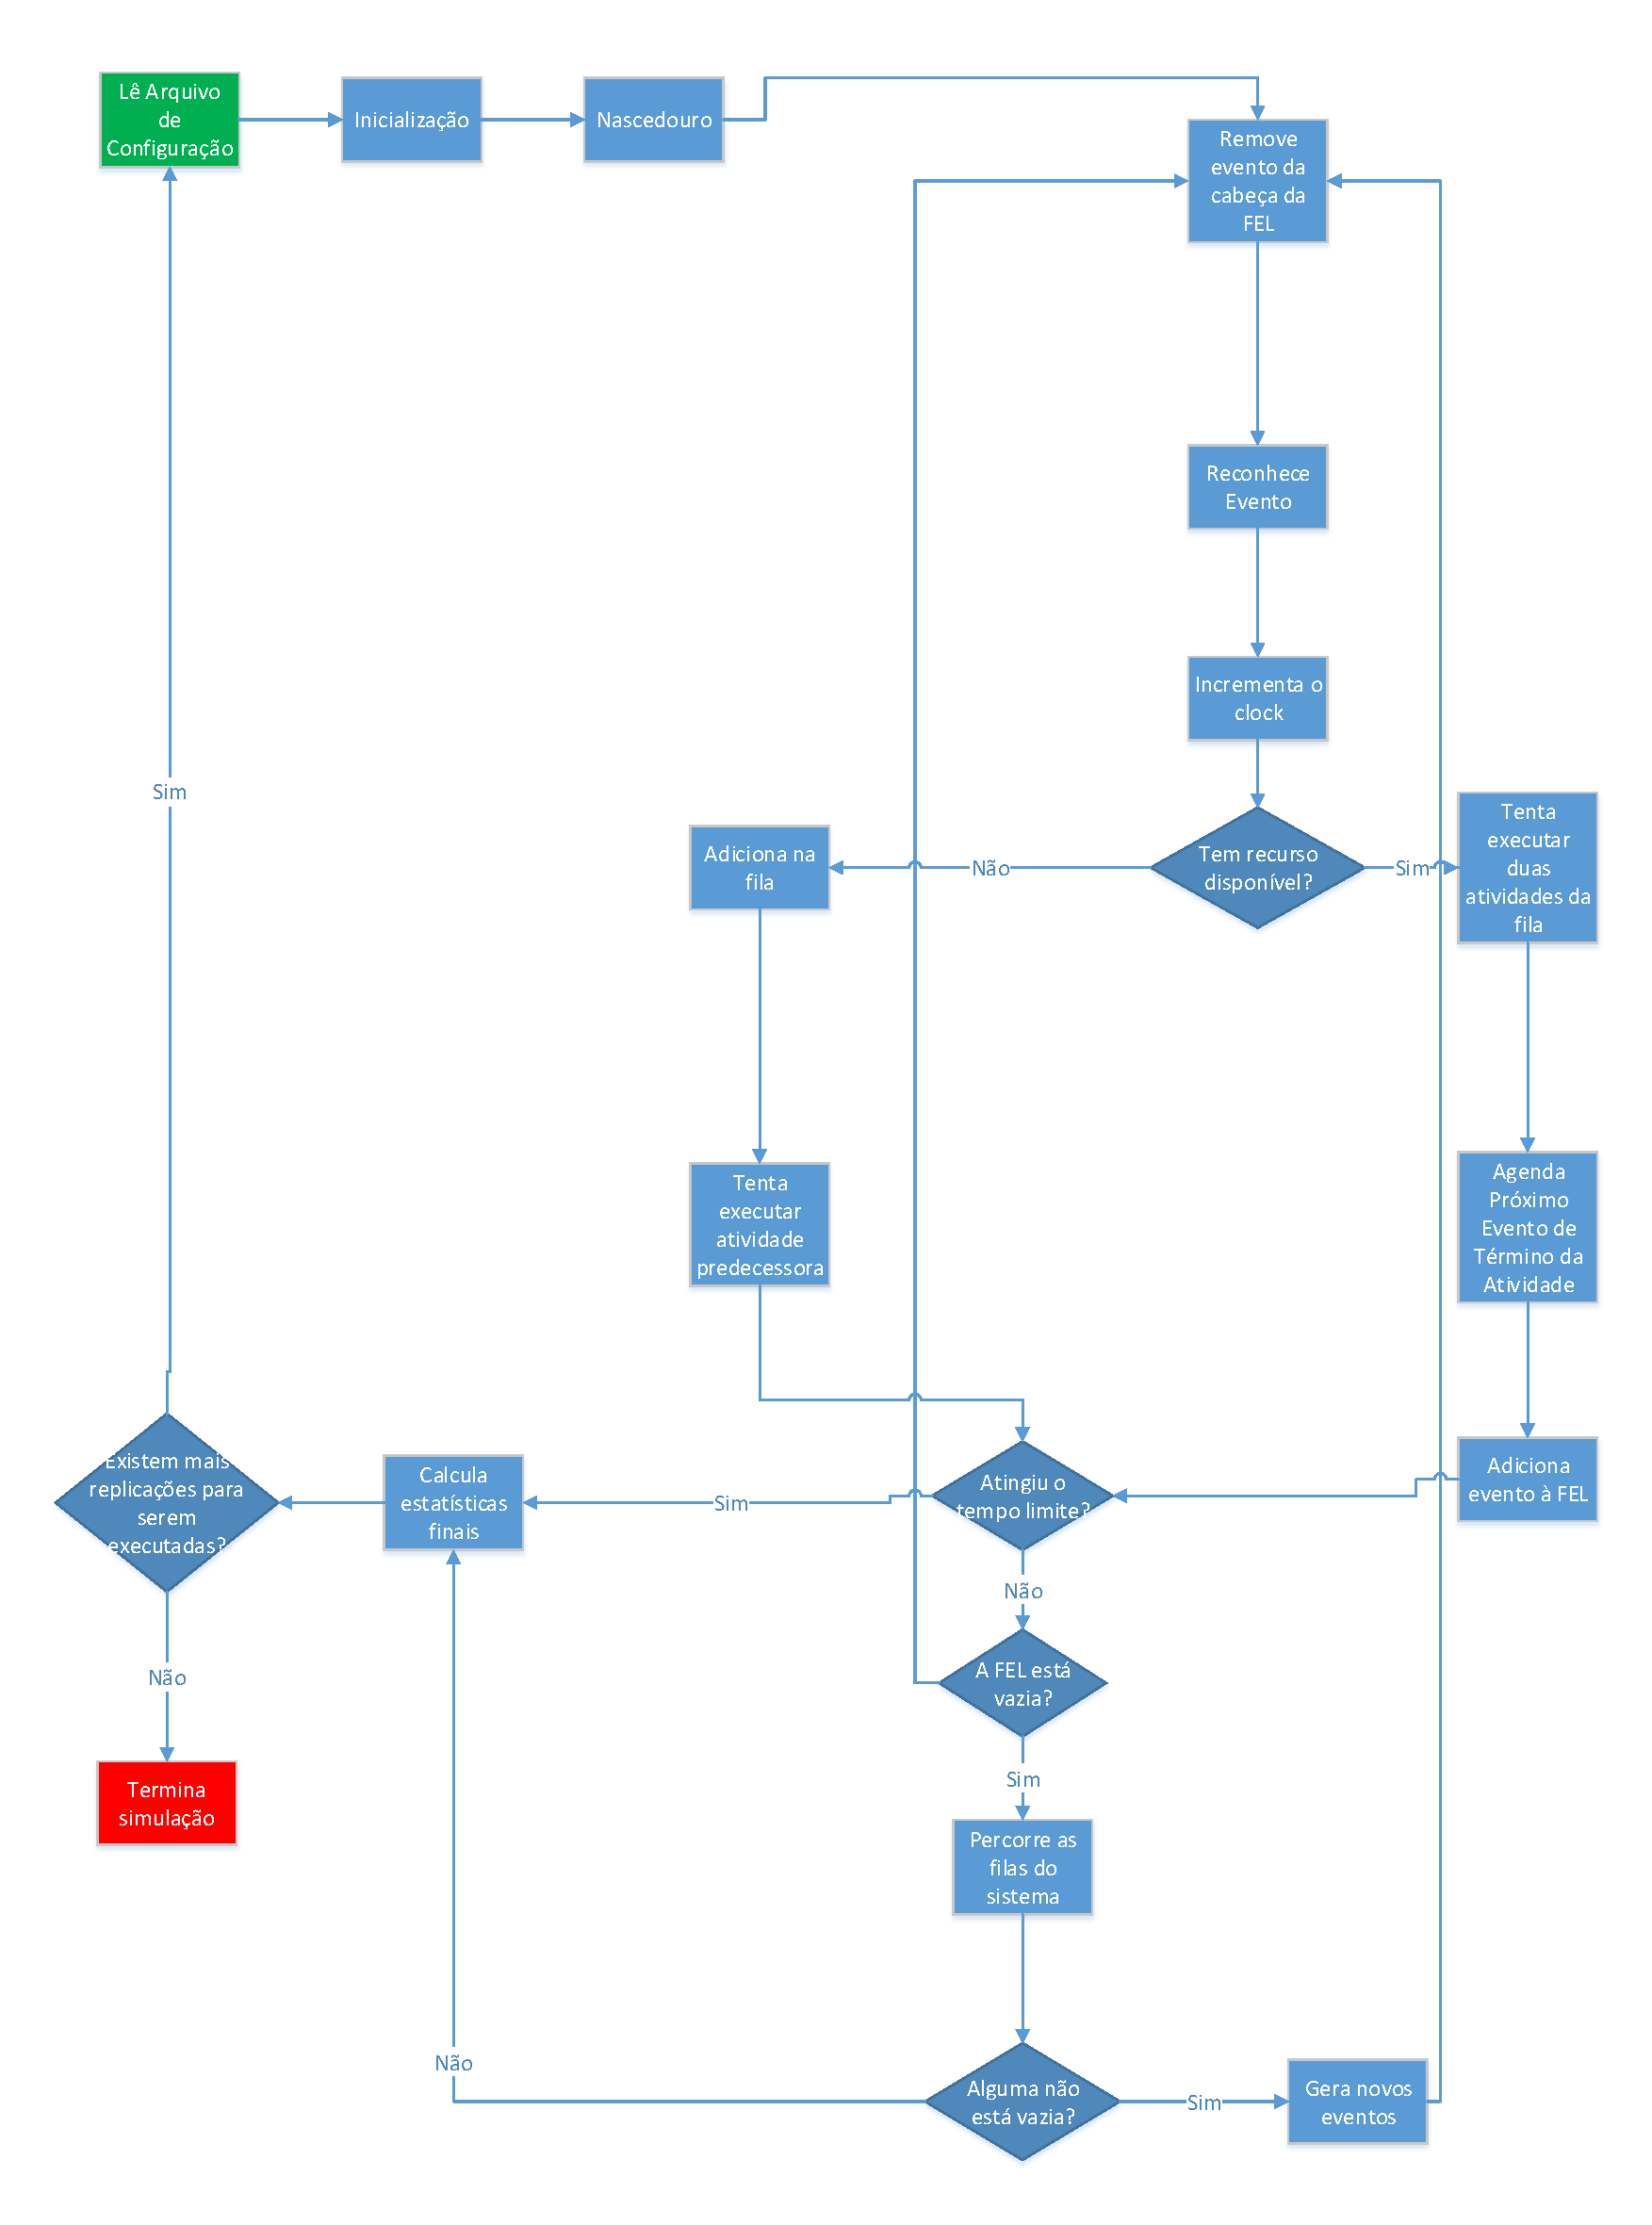
\includegraphics[width=0.5\linewidth]{model.pdf}
\end{frame}
	
\subsection{Entrada de Dados}
	
\begin{frame}{}
	\centering
	\Huge \color{blue} \textbf{Entrada de Dados}
\end{frame}
	
\begin{frame}{Entrada de Dados}
	\begin{itemize}
		\item A aplicação recebe três parâmetros:
		      \bigskip
		      \begin{itemize}
		      	\item \textbf{\textit{in}}: Arquivo de configuração;
		      	      \bigskip
		      	\item \textbf{\textit{out}}: Nome do arquivo de estatísticas de saída;
		      	      \bigskip
		      	\item \textbf{\textit{debug}}: Tipo de mensagens de depuração que serão mostradas.
		      	      \bigskip
		      \end{itemize}
	\end{itemize}
\end{frame}
	
\begin{frame}{Arquivo de configuraçao}
	\begin{itemize}
		\item Definido por um conjunto de tag's:
		      \bigskip
		      \begin{itemize}
		      	\item \textbf{c}: Comentário;
		      	      \bigskip
		      	\item \textbf{n}: Quantidade de replicações;
		      	      \bigskip
		      	\item \textbf{t}: Tempo máximo de simulação, em minutos;
		      	      \bigskip
		      	\item \textbf{p}; Quantidade de pedidos a chegar;
		      \end{itemize}
	\end{itemize}
\end{frame}
	
\begin{frame}{Arquivo de configuraçao - Entidades}
	\begin{itemize}
		\item {\tt funcSetorCompra <num>}
		      \medskip
		\item {\tt funcSetorExpedicao <num>}
		      \medskip
		\item {\tt funcSetorModel <num>}
		      \medskip
		\item {\tt funcSetorProducao <num>}
		      \medskip
		\item {\tt funcProdManual <num>}
		      \medskip
		\item {\tt funcSetorFinal <num>}
		      \medskip
		\item {\tt funcCheckoutResina <num>}
		      \medskip
		\item {\tt funcSetorQualidade <num>}
		      \medskip
		\item {\tt funcSetorContProd <num>}
		      \medskip
		\item {\tt funcSetorDoc <num>}
		      \medskip
		\item {\tt servTerc <num>}
	\end{itemize}
\end{frame}
	
	
\begin{frame}{Arquivo de configuraçao - Duração das atividades}
	\begin{itemize}
		\item  {\tt <distribuição>\_<nome-atividade>\_<parâmetro> <num> }
		      \bigskip
		\item Distribuições disponíveis e seus parâmetros:
		      \bigskip
		      \begin{itemize}
		      	\item norm:
		      	      \begin{itemize}
		      	      	\item med
		      	      	\item sd
		      	      \end{itemize}
		      	\item tri:
		      	      \begin{itemize}
		      	      	\item min
		      	      	\item med
		      	      	\item max
		      	      \end{itemize}
		      	\item unif:
		      	      \begin{itemize}
		      	      	\item min
		      	      	\item max
		      	      \end{itemize}
		      \end{itemize}
		      \bigskip
		\item Constantes: {\tt cte\_<nome-atividade> <num>}
	\end{itemize}
\end{frame}
	
\begin{frame}{Arquivo de configuraçao - Exemplo}
	\begin{block}{Exemplo de arquivo de configuração}
		{\footnotesize
			{\color{red} \textbf{c} Quantidade de replicações}\\
			\textbf{n} 1000000\\
			{\color{red} \textbf{c} Tempo máximo de simulação em minutos}\\
			\textbf{t} 57600\\
			{\color{red} \textbf{c} Quantidade de pedidos a chegar}\\
			\textbf{p} 15\\
			{\color{red} \textbf{c} Quantidades de cada entidade }\\
			\textbf{funcSetorCompra} 2\\
			\textbf{servTerc} 1\\
			{\color{red} \textbf{c} Duração das atividades }\\
			\textbf{norm\_cheg\_ped\_med} 120\\
			\textbf{norm\_cheg\_ped\_sd} 40\\
						
			\textbf{tri\_proc\_exp\_ped\_min} 30\\
			\textbf{tri\_proc\_exp\_ped\_med} 40\\
			\textbf{tri\_proc\_exp\_ped\_max} 180\\
						
			\textbf{unif\_verif\_data\_mat\_prim\_min} 15\\
			\textbf{unif\_verif\_data\_mat\_prim\_max} 45\\
						
			\textbf{cte\_id\_mat} 10
		}
	\end{block}
\end{frame}
	
\begin{frame}[allowframebreaks]{Opções de depuração}
	\begin{itemize}
		\item A depuração no processo de simulação é importante, porém é um pouco complexa:
        \bigskip
		      \begin{itemize}
		      	\item Existem muitas ações simultâneas;
		      	      \bigskip
		      	\item É difícil acompanhar o \aspas{Cilo de vida} de uma entidade;
		      	      \bigskip
		      	\item No sistema desenvolvido, existem muitas atividades e tipos de eventos.
		      \end{itemize}
		      \bigskip
		      \framebreak
		\item Foi desenvolvido um sistema de depuração controlado por parâmetros, facilitando a manutenção e inspeção da aplicação;
		      \bigskip
		\item Depuração definida pela opção \texttt{debug= <opção1,opção2,...>};
		      \bigskip
		\item Opções disponíveis:
		      \begin{itemize}
		      	\item \textbf{info}: informações de execução da simulação (início e término de uma replicação, estatísticas gerais, ...);
		      	      \bigskip
		      	\item \textbf{entidade}: informações das entidades do sistema (atribuição e liberação de funcionários, ...);
		      	      \bigskip
		      	\item \textbf{fila}: informações das filas do sistema (quem saiu/entrou na fila X, tamanho atual da fila, ...);
		      	      \bigskip
		      	\item \textbf{evento}: informações dos eventos criados no sistema;
		      	      \bigskip
		      	\item \textbf{tudo}: ativa todas as opções de depuração.
		      \end{itemize}
	\end{itemize}
\end{frame}
	
	
\subsection{Alternativas de Cenários}
	
\begin{frame}{}
	\centering
	\Huge \color{blue} \textbf{Alternativas de Cenários}
\end{frame}
	
\begin{frame}{Cenário 1 (C1)}
	\label{fram:cenario1}
	\begin{itemize}
		\item  Foi duplicada a quantidade de entidades e manteve-se a quantidade de serviços de terceiros;
		      \bigskip
		\item Teve-se a intenção de verificar se a fila de Serviço Terceirizado era realmente o gargalo do modelo:
        \medskip
		      \begin{itemize}
		      	\item Com mais funcionários nas atividades precedentes, mais pedidos chegam até a atividade de Serviço Terceirizado.
		      \end{itemize}
	\end{itemize}
\end{frame}	
		
\begin{frame}{Cenário 2 (C2)}
	\label{fram:cenario2}
	\begin{itemize}
		\item Foi duplicada a quantidade de entidades e foi quadruplicada a quantidade de serviços de terceiros;
		      \bigskip
		\item Foi observado no primeiro cenário (slide \ref{fram:cenario1}) que o gargalo do sistema era realmente o Serviço Terceirizado;
		      \bigskip
		\item Fez-se a suposição de que aumentando a quantidade de serviços de terceiros, tal gargalo seria reduzido;
		      \bigskip
		\item Na vida real seria a contratação de mais empresas terceirizadas ou o contrato de mais serviços de uma mesma empresa.
	\end{itemize}
\end{frame}	
		
\begin{frame}{Cenário 3 (C3)}
	\label{fram:cenario3}
	\begin{itemize}
		\item Foram observados no ACD, os setores onde os funcionários estavam mais sobrecarregados;
		      				
		      \bigskip
		      				
		      \begin{itemize}
		      	\item Atribuídos à muitas atividades;
		      	      					
		      	      \bigskip
		      	      					
		      	\item Atribuídos à atividades com longa duração;
		      \end{itemize}
	\end{itemize}
\end{frame}	
		
\begin{frame}{Cenário 3 (C3)}
	\begin{itemize}
		\item Funcionários do setor de compra: 2
		\item Funcionários do setor de Expedição: 2
		\item Funcionários do setor de Modelação: 4
		\item Funcionários do setor de Produção: 2
		\item Funcionários do setor de Produção Manual: 2
		\item Funcionários do setor de Finalização: 2
		\item Funcionários do setor de Limpeza Especial: 4
		\item Funcionários do setor de Qualidade: 5
		\item Funcionários do setor de Continuação de Produção: 2
		\item Funcionários do setor de Documentação: 3
		\item Quantidade de serviços de terceiros: 4
	\end{itemize}
\end{frame}	

\begin{frame}{Cenário 4 (C4)}
	\label{fram:cenario4}
	\begin{itemize}
		\item Foi duplicada a quantidade de entidades e foi multiplicada por 8 a quantidade de serviços de terceiros;
		      \bigskip
		\item Foi observado no primeiro cenário (slide \ref{fram:cenario1}) que o gargalo do sistema era realmente o Serviço Terceirizado;
		      \bigskip
		\item Fez-se a suposição de que aumentando a quantidade de serviços de terceiros, tal gargalo seria reduzido;
		      \bigskip
		\item Esse cenário implica em um maior custo financeiro.
	\end{itemize}
\end{frame}	
		
\subsection{Experimentação}
	
\begin{frame}{Experimentação}
	\begin{itemize}
		\item Devido ao curto tempo da simulação de uma replicação, foi utilizado $n=1.000.000$ para a amostra piloto;
		      			
		      \bigskip
		      			
		\item A precisão $h^*$ escolhida foi de 120 minutos:
        \medskip
		      \begin{itemize}
		      	\item A escala de todo o sistema é de minutos;
		      	      \bigskip
		      	\item Certas atividades levam horas e até mesmo dias para serem executados, então foi considerada uma precisão justa.
		      \end{itemize}
		      			
		      \bigskip
		      			
		\item O $n^*$ (i. e. rodadas para alcançar a precisão desejada) só é calculado caso o tamanho do intervalo de confiança ($H$) da amostra piloto já não tenha alcançado a precisão desejada;
		      			
		      \bigskip
		      			
		\item Foi necessário o cálculo de $n^*$ apenas na comparação dos cenários, onde encontrou-se $n^*=1.466.188$, sendo esse o maior dos $n^*$ encontrados. 
	\end{itemize}
			
\end{frame}
	
\begin{frame}{Experimentação - Cálculo do intervalo de confiança}
	\begin{itemize}
		\item Para cálculo do intervalo de confiança, são realizadas as seguintes operações:
        		\medskip
		      \begin{itemize}
		      	\item Cálculo da confiança estatística: $ prob = 1 - \frac{\alpha}{2} $
                \bigskip
		      	\item Onde $\alpha$ é a confiança desejada. Ex: $\alpha=0.05$ leva a uma confiança de 95\%;
		      	      \bigskip
		      	\item Calculo da amplitude $H$ do intervalo de confiança: $ t_{n-1, prob}\frac{s}{\sqrt{n}} $
                \bigskip
		      	\item Onde:
		      	      \begin{itemize}
		      	      	\item $t_{n-1, prob}$ é o percentil $(1-\alpha/2)$ da distribuição $t$ de Student com $(n-1)$ graus de liberdade;
                        \medskip
		      	      	\item $s$ é o desvio padrão da amostra;
                        \medskip
		      	      	\item $n$ é o tamanho da amostra.
                        \medskip
		      	      \end{itemize}
		      	\item O intervalo de confiança corresponde à $[\overline{x}-H ; \overline{x}+H]$
		      \end{itemize}
	\end{itemize}
\end{frame}
	
\begin{frame}{Exeperimentação - Cálculo do intervalo de confiança}
	\begin{itemize}
		\item Caso o $H$ não atinja a precisão desejada ($h^*$), é preciso calcular as $n^*$ replicações adicionais para se alcançar a precisão: $$ n^* = \ceil*[\big]{n\left(\frac{h}{h^*}\right)^2 }$$
	\end{itemize}
\end{frame}
	
\begin{frame}{Exeperimentação - Comparação de amostras $N$ iguais}
	\begin{itemize}
		\item Calcula-se a diferença das duas amostras;
		      \bigskip
		\item Dada a amostra de diferença, repete o procedimento do cálculo do intervalo de confiança, tomando $\theta_{1}=\overline{x}-H$ e $\theta_{2}=\overline{x}+H$;
		      \bigskip
		\item Seguindo, são possíveis os seguintes resultados:
		      \begin{itemize}
		      	\item $\theta_{1}<0$ e $\theta_{2}>0$: Nada se pode afirmar sobre as médias das amostras;
		      	      \bigskip
		      	\item $\theta_{1}>0$ e $\theta_{2}>0$: A média da Amostra 1 é maior do que a média da Amostra 2;
		      	      \bigskip
		      	\item $\theta_{1}<0$ e $\theta_{2}<0$: A média da Amostra 2 é maior do que a média da Amostra 1;
		      \end{itemize}
	\end{itemize}
\end{frame}
	
\begin{frame}{Exeperimentação - Tempo de Simulação Total}
	\begin{itemize}
		\item O tempo de simulação total de cada cenário foi considerado como o tempo de simulação + operações de Entrada/Saída e outras operações feitas pela aplicação;
		      				
		      \bigskip
		      				
		\item Para tal, foi utilizado o comando \texttt{time}\footnote{\url{http://man7.org/linux/man-pages/man2/time.2.html}} do Linux.
	\end{itemize}
			
	\begin{table}[H]
		\centering
		\begin{tabular}{|c|c|}
			\hline
			\textbf{Cenários}        & \textbf{Tempo total} \\ \hline
			Cenário \textit{default} & 24m                  \\ \hline
			Cenário 1                & 25m                  \\ \hline
			Cenário 2                & 27m                  \\ \hline
			Cenário 3                & 29m                  \\ \hline
			Cenário 4                & 31m                  \\ \hline
		\end{tabular}
		\caption {Tempo total de simulação de cada cenário}
	\end{table}
				
\end{frame}
		
\section{Resultados}

\begin{frame}{}
	\centering
	\Huge \color{blue} \textbf{Resultados}
\end{frame}

\begin{frame}{Tempo médio em fila de Serviços de Terceiros}
	\begin{table}[H]
		\centering
		\begin{tabular}{|c|c|c|c|}
			\hline
			\textbf{Cenários} & \textbf{Média (minutos)}\footnotemark & \textbf{SD (minutos) }\footnotemark & \textbf{H} \\ \hline
			CD                 & 157061.7 (109 dias)                    & 57283.03 (40 dias)                  & 92.72133   \\ \hline
			C1                 & 134692.5 (94 dias)                     & 47035.45 (33 dias)                  & 76.13405   \\ \hline
			C2                 & 86623.02 (61 dias)                     & 33432.44 (24 dias)                  & 54.1155    \\ \hline
			C3                 & 92694.62 (64 dias)                     & 33949.51 (24 dias)                  & 54.95246   \\ \hline
			C4                 & 46876.29 (33 dias)                     & 22400.84 (16 dias)                  & 36.25918   \\ \hline
		\end{tabular}
		\caption {Tempo de espera na fila de Serviços Terceirizados}
	\end{table}
	\footnotetext{As medidas de dispersão ficaram muito altas devido à quantidade de \textit{outliers} nas amostras obtidas.}
\end{frame}

\begin{frame}{Tempo médio em fila de Serviços de Terceiros}
	\begin{figure}[H]
		\centering
		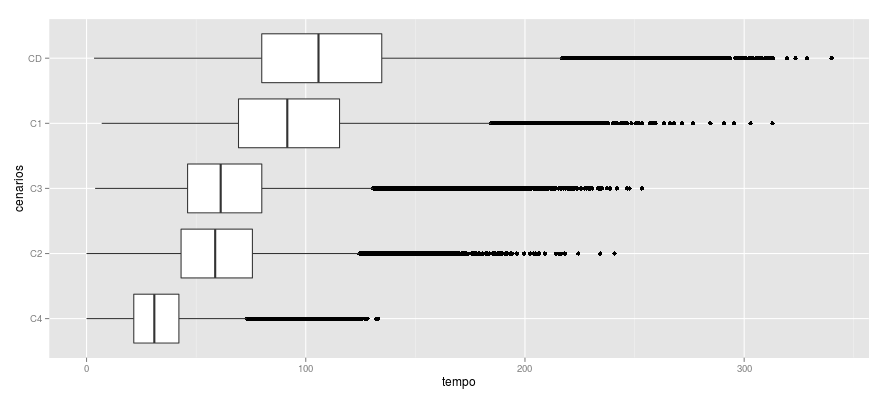
\includegraphics[width=1\linewidth]{img/final.png}
		\caption{Tempo médio de espera na fila de terceiros}
		\label{fig:box}
	\end{figure}
\end{frame}
	
\begin{frame}{Tempo médio em fila de Serviços de Terceiros}
	\begin{itemize}
		\item Olhando os histogramas, os dados parecem seguir uma distribuição Normal ou Weibull;
        \bigskip
        \item Tal afirmação pode ser verificada plotando os histogramas em relação às curvas teóricas das distribuições.
	\end{itemize}
\end{frame}
	
\begin{frame}{Tempo médio em fila de Serviços de Terceiros}
	\begin{figure}[H]
		\centering
		\begin{subfigure}[H]{0.4\textwidth}
			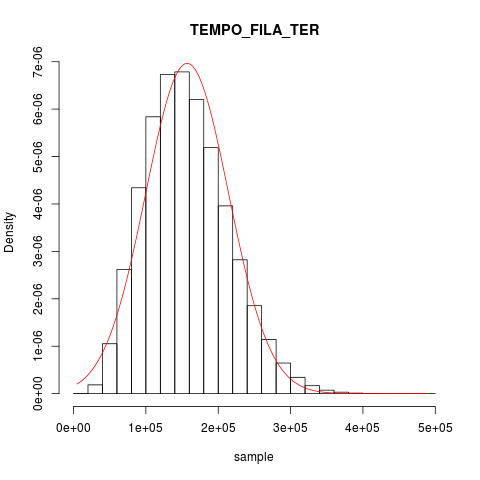
\includegraphics[width=\textwidth]{img/CD-hist-norm-TEMPO_FILA_TER.png}
			\caption{Comparação com a curva teórica da distribuição Normal}
			\label{fig:CD-norm}
		\end{subfigure}
		%
		\begin{subfigure}[H]{0.4\textwidth}
			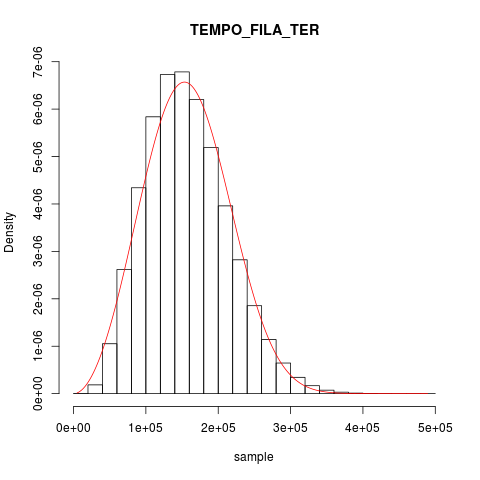
\includegraphics[width=\textwidth]{img/CD-hist-weibull-TEMPO_FILA_TER.png}
			\caption{Comparação com a curva teórica da distribuição Weibull}
			\label{fig:CD-wei}
		\end{subfigure}
		\caption{Curvas teóricas e dados coletados do cenário \textit{Default}}
	\end{figure}
\end{frame}
	
\begin{frame}{Tempo médio em fila de Serviços de Terceiros}
	\begin{figure}[H]
		\centering
		\begin{subfigure}[H]{0.4\textwidth}
			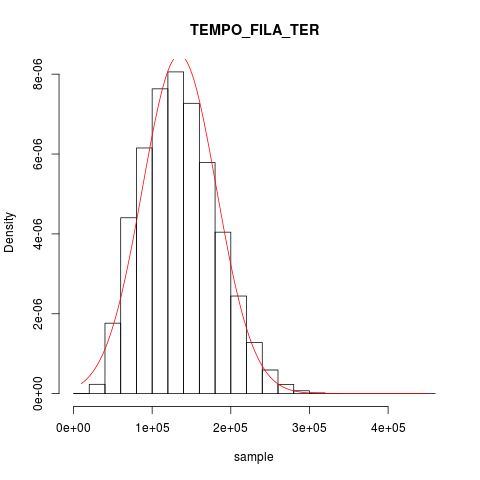
\includegraphics[width=\textwidth]{img/C1-hist-norm-TEMPO_FILA_TER.png}
			\caption{Comparação com a curva teórica da distribuição Normal}
			\label{fig:C1-norm}
		\end{subfigure}
		%
		\begin{subfigure}[H]{0.4\textwidth}
			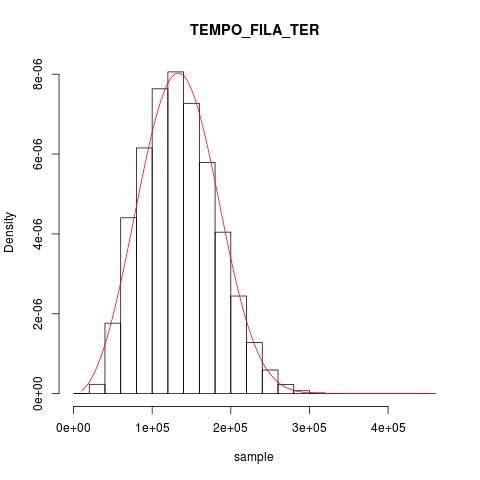
\includegraphics[width=\textwidth]{img/C1-hist-weibull-TEMPO_FILA_TER.png}
			\caption{Comparação com a curva teórica da distribuição Weibull}
			\label{fig:C1-wei}
		\end{subfigure}
		\caption{Curvas teóricas e dados coletados do cenário 1}
	\end{figure}
\end{frame}
	
\begin{frame}{Tempo médio em fila de Serviços de Terceiros}
	\begin{figure}[H]
		\centering
		\begin{subfigure}[H]{0.4\textwidth}
			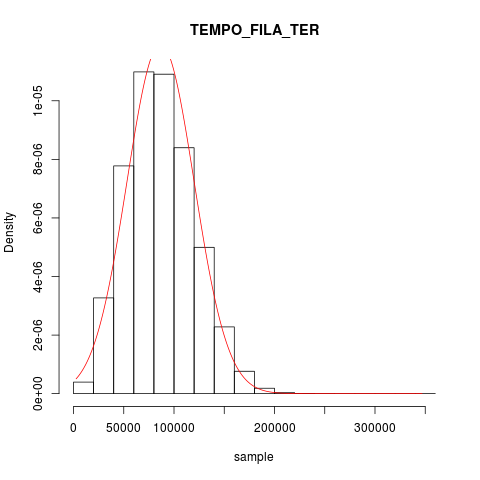
\includegraphics[width=\textwidth]{img/C2-hist-norm-TEMPO_FILA_TER.png}
			\caption{Comparação com a curva teórica da distribuição Normal}
			\label{fig:C2-norm}
		\end{subfigure}
		%
		\begin{subfigure}[H]{0.4\textwidth}
			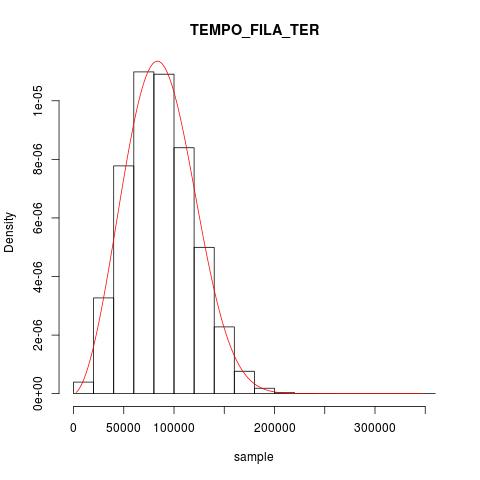
\includegraphics[width=\textwidth]{img/C2-hist-weibull-TEMPO_FILA_TER.png}
			\caption{Comparação com a curva teórica da distribuição Weibull}
			\label{fig:C2-wei}
		\end{subfigure}
		\caption{Curvas teóricas e dados coletados do cenário 2}
	\end{figure}
\end{frame}
	
\begin{frame}{Tempo médio em fila de Serviços de Terceiros}
	\begin{itemize}
		\item Já o cenário 3 apresenta maior semelhança com a distribuição \textbf{LogNormal}:
	\end{itemize}
	\begin{figure}[H]
		\centering
		\begin{subfigure}[H]{0.4\textwidth}
			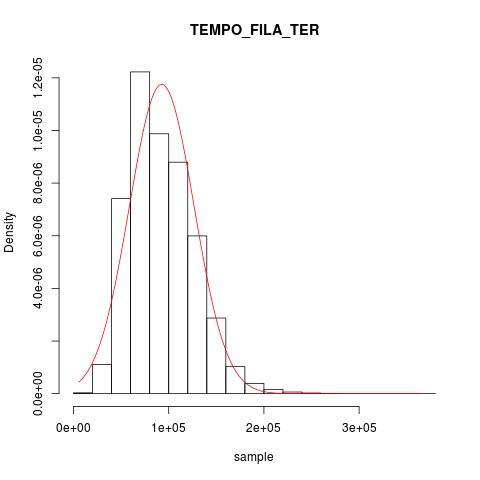
\includegraphics[width=\textwidth]{img/C3-hist-norm-TEMPO_FILA_TER.png}
			\caption{Comparação com a curva teórica da distribuição Normal}
			\label{fig:C3-norm}
		\end{subfigure}
		%
		\begin{subfigure}[H]{0.4\textwidth}
			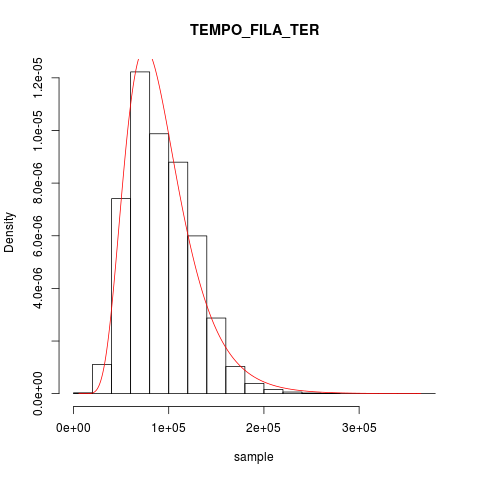
\includegraphics[width=\textwidth]{img/C3-hist-lnorm-TEMPO_FILA_TER.png}
			\caption{Comparação com a curva teórica da distribuição \textbf{LogNormal}}
			\label{fig:C3-logn}
		\end{subfigure}
		\caption{Curvas teóricas e dados coletados do cenário 3}
	\end{figure}
\end{frame}

\begin{frame}{Tempo médio em fila de Serviços de Terceiros}
	\begin{figure}[H]
		\centering
		\begin{subfigure}[H]{0.4\textwidth}
			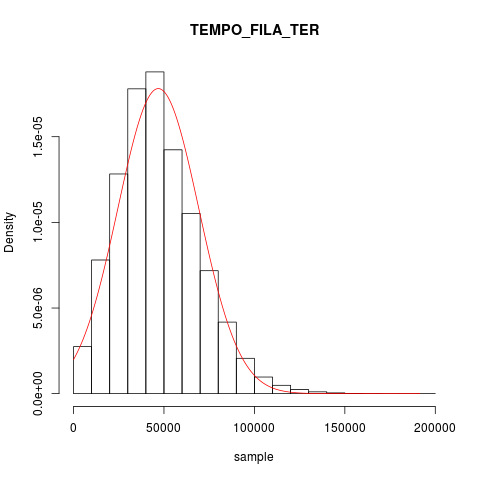
\includegraphics[width=\textwidth]{img/C4-hist-norm-TEMPO_FILA_TER.png}
			\caption{Comparação com a curva teórica da distribuição Normal}
			\label{fig:C4-norm}
		\end{subfigure}
		%
		\begin{subfigure}[H]{0.4\textwidth}
			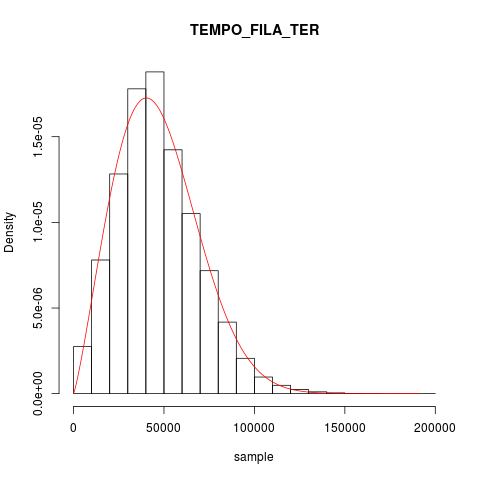
\includegraphics[width=\textwidth]{img/C4-hist-weibull-TEMPO_FILA_TER.png}
			\caption{Comparação com a curva teórica da distribuição Weibull}
			\label{fig:C4-wei}
		\end{subfigure}
		\caption{Curvas teóricas e dados coletados do cenário 4}
	\end{figure}
\end{frame}
	
\begin{frame}{Estatísticas de cada cenário}
	\begin{itemize}
		\item \textbf{TRS}: Tempo real de simulação, desconsiderando operações de Entrada/Saída e não relacionadas a simulação;
        \medskip
		\item \textbf{PA}: Pedidos Atendidos, quantidade de pedidos atendidos ao final da simulação.
	\end{itemize}
	\begin{table}[H]
		\centering
		\begin{tabular}{|c|c|c|c|c|}
			\hline
			\textbf{Cenários} & \textbf{TRS - Média (ms)} & \textbf{PA (min)} & \textbf{PA (max)} & \textbf{PA (mean)} \\ \hline
			CD                 & 0.12                       & 1                 & 7                 & 1                  \\ \hline
			C1                 & 0.13                       & 1                 & 7                 & 1                  \\ \hline
			C2                 & 0.13                       & 4                 & 11                & 4                  \\ \hline
			C3                 & 0.14                       & 4                 & 12                & 4                  \\ \hline
			C4                 & 0.15                       & 8                 & 15                & 9                  \\ \hline
		\end{tabular}
		\caption {Estatísticas de cada cenário}
	\end{table}
\end{frame}
	
\begin{frame}{Intervalo de Confiança de cada cenário}
	\begin{table}[H]
		\centering
		\begin{tabular}{|c|c|}
			\hline
			\textbf{Cenários} & \textbf{Intervalo de Confiança} \\ \hline
			Cenário Default   & [ 156969 - 157154.4 ]            \\ \hline
			Cenário 1         & [ 134616.3 - 134768.6 ]          \\ \hline
			Cenário 2         & [ 86568.91 - 86677.14 ]          \\ \hline
			Cenário 3         & [ 92639.67 - 92749.57 ]          \\ \hline
			Cenário 4         & [ 46840.03 - 46912.55 ]          \\ \hline
		\end{tabular}
		\caption {Intervalo de Confiança de cada cenário}
	\end{table}
\end{frame}
	
\begin{frame}{Comparação de alternativas simuladas}
	\begin{table}[H]
		\centering
		\begin{tabular}{|c|c|c|c|}
			\hline
			\textbf{Cenários} & \textbf{Amostra 1} & \textbf{Amostra 2} & \textbf{H} \\ \hline
			CD X C1            & ~                  & X                  & 119.9772  \\ \hline
			CD X C2            & ~                  & X                  & 107.3631   \\ \hline
			CD X C3            & ~                  & X                  & 107.8317    \\ \hline
			CD X C4            & ~                  & X                  & 99.50416    \\ \hline
			C1 X C2            & ~                  & X                  & 93.45891     \\ \hline
			C1 X C3            & ~                  & X                  & 93.85324     \\ \hline
			C1 X C4            & ~                  & X                  & 84.28417     \\ \hline
			C2 X C3            & X                  & ~                  & 77.14725    \\ \hline
			C2 X C4            & ~                  & X                  & 65.18329      \\ \hline
			C3 X C4            & ~                  & X                  & 65.8403      \\ \hline
		\end{tabular}
		\caption {Comparação de alternativas simuladas}
	\end{table}
\end{frame}
	
\section{Conclusões}

\begin{frame}{}
	\centering
	\Huge \color{blue} \textbf{Conclusões}
\end{frame}
	
\begin{frame}{Conclusões}
	\begin{itemize}
		\item Observando as médias, o Cenário 4 apresenta a menor média de tempo de espera em fila de Serviços de Terceiros, analisando o indicador de desempenho em questão, esse é o \textbf{melhor cenário};
		      			
		      \bigskip
		      			
		\item Pelas médias cruas, o Cenário 4 possui um tempo média de espera mais de 3 vezes menor que o Cenário \textit{Default}: 
		      			
		      \begin{block}{}
		      	$$ mediaCD: 157061.7/ mediaC4: 46876.29 = \textbf{3.350557393} $$
		      \end{block}
		      	
         \medskip
		\item Analisando a quantidade de pedidos atendidos, o Cenário 4 também apresenta uma média superior, atendendo em média 9 peças e chegando a atender até mesmo as 15 peças que chegaram, no mesmo intervalo de tempo.
		      
	\end{itemize}		
\end{frame}
	
\begin{frame}{Conclusões}
	\begin{itemize}
		\begin{block}{Contratar mais serviços de empresas terceirizadas, reduz o tempo de espera na fila de Serviços Terceirizados?}
			Talvez o ato de pagar um pouco mais caro por mais serviços possa gerar mais lucro pelo fato de diminuir o gargalo na fila de espera do serviço de terceiros, levando ao atendimento de mais pedidos;
		\end{block}
					
		\bigskip
					
		\item Caso a administração da Fundição California tenha condições financeiras, é interessante contratar mais serviços de terceiros, atendendo mais clientes no mesmo tempo e reduzindo o tempo em fila.
	\end{itemize}		
\end{frame}

\frame{\titlepage}
\end{document}
